La fase de diseño consiste en aplicar una serie de técnicas para transformar los requisitos elicitados en la fase de análisis en una estructura detallada para el sistema de forma que se pueda implementar fácilmente a partir de ese diseño.\\

Siguiendo los requisitos de la fase anterior, esta tarea es relativamente sencilla y debe resultar en una serie de diagramas y especificaciones que sirvan como guión y documentación a las personas que vayan a participar, ahora o en un futuro en el desarrollo del sistema.\\

La aplicación se rige por el patrón arquitectónico MVC. La capa del modelo equivale al SGBD y al ORM, mientras el controlador es el responsable de hacer de intermediario entre vista y modelo, llevando la lógica de la aplicación. Las vistas serán los ficheros XHTML junto con sus estilos.

\section{Controladores}

A continuación, se comentarán las acciones más importantes que componen cada uno de los controladores. Normalmente cada controlador tiene asociado un modelo, y cada acción del controlador una vista.

\subsection{Users}

Controlador encargado de llevar toda la gestión de usuarios

\begin{itemize}
\item users::add() - Muestra el formulario de creación de un usuario.
\item users::create() - Crea un usuario según los datos introducidos en el formulario.
\item users::edit() - Muestra un formulario con los datos del usuario a editar sobre él para poder ser modificados.
\item users::update() - Actualiza un usuario segun los datos introducidos.
\item users::recuperar\_password() - Muestra el formulario para recuperar una contraseña.
\item users::envio\_recuperar() - Envía y cambia la contraseña a un usuario por email a la dirección introducida en el formulario.
\end{itemize}

\subsection{Login}

Controlador encargado de gestionar la identificación de usuarios en el sistema.

\begin{itemize}
\item login::index() - Muestra el formulario de solicitud de datos de acceso.
\item login::submit() - Comprueba los datos introducidos en el formulario anterior e identifica al usuario si son correctos, sino recarga el formulario y lo indica.
\end{itemize}

\subsection{Logout}

Controlador encargado de gestionar la salida de los usuarios del sistema

\begin{itemize}
\item logout::index() - Provoca la salida del usuario del sistema.
\end{itemize}

\subsection{Admin}

Controlador encargado de algunas funciones de administración.

\begin{itemize}
\item admin::restaurar\_backup() - Muestra un formulario para cargar un archivo sql con una copia de seguridad de la base de datos, restaurando los datos que estuvieran en ese archivo.
\item admin::restaurar() - Restaura la base de datos con el archivo cargado en el formulario anterior.
\item admin::backup() - Permite la descarga de un backup del estado actual de la base de datos.
\end{itemize}

\subsection{Titulaciones}
Controlador encargado de llevar a cabo toda la gestión de las titulaciones.

\begin{itemize}
\item titulaciones::index() - Muestra las titulaciones que hay creadas en el sistema.
\item titulaciones::show\_informes() - Muestra un listado de las asignaturas de la titulación permitiendo generar un informe con las que se quieran seleccionar.
\item titulaciones::add() - Muestra un formulario de creación de titulaciones.
\item titulaciones::create() - Crea una titulación a partir de los datos introducidos en el formulario.
\item titulaciones::edit() - Permite la edición de una titulación mostrando un formulario.
\item titulaciones::update() - Actualiza los datos de una titulación existente.
\item titulaciones::delete() - Borra una titulación del sistema.
\item titulaciones::show() - Muestra las asignaturas de esa titulación.
\item titulaciones::show\_planificacion() - Muestra una tabla con la planificación docente de una titulación, con una fila por asignatura.
\item titulaciones::exportar\_planificacion() - Permite la descarga de un archivo csv con la planificación docente completa de todas las asignaturas de la titulación.
\item titulaciones::select\_titulacion() - Muestra un listado de las titulaciones permitiendo enrutar hacia a otra acción que necesite seleccionar una titulación.
\end{itemize}

\subsection{Asignaturas}
Controlador encargado de llevar a cabo toda la gestión de las asignaturas.

\begin{itemize}
\item asignaturas::show() - Muestra la planificación docente de una asignatura para un curso concreto.
\item asignaturas::add\_to() - Añade una asignatura a una titulación dada mostrando un formulario.
\item asignaturas::create() - Crea una asignatura siguiendo los datos introducidos en el formulario.
\end{itemize}

\subsection{Aulas}
Controlador encargado de llevar a cabo la gestión de las aulas.

\begin{itemize}
\item aulas::add() - Muestra el formulario de creación de un aula.
\item aulas::create() - Crea un aula a partir de los datos introducidos en el formulario.
\item aulas::index() - Muestra un listado de todas las aulas.
\item aulas::exportar\_ocupacion() - Exporta a un archivo csv la ocupación de un aula según los horarios de un curso concreto.
\end{itemize}

\subsection{Cursos}

Controlador que lleva toda la gestión de los cursos.

\begin{itemize}
\item cursos::add() - Muestra el formulario para la creación de un curso nuevo.
\item cursos::create() - Crea un curso con los datos introducidos.
\item cursos::edit() - Muestra un formulario para editar un curso ya creado.
\item cursos::update() - Actualiza un curso existente con los datos introducidos.
\item cursos::delete() - Borra un curso existente.
\item cursos::select\_curso() - Muestra un listado de los cursos permitiendo enrutar hacia a otra acción que necesite seleccionar uno.
\end{itemize}

\subsection{Eventos}

Controlador encargado de la gestión del calendario.

\begin{itemize}
\item eventos::index() - Muestra el calendario del sistema permitiendo crear nuevos eventos sobre el.
\item eventos::add() - Muestra un formulario para la creación de eventos.
\item eventos::create() - Crea un evento con los datos introducidos en el formulario.
\item eventos::delete() - Borra un evento existente.
\item eventos::fetch\_events() - Función que devuelve en formato JSON los datos de los eventos del sistema para mostrarlos sobreimpresos en el calendario.
\item eventos::export\_calendar() - Exporta y permite la descarga del calendario en formato csv.
\end{itemize}

\subsection{Horarios}

Controlador encargado de la gestión de los horarios.

\begin{itemize}
\item horarios::select\_grupo() - Muestra los cursos de una titulación y sus grupos creados, con enlaces a los diferentes horarios.
\item horarios::add\_grupo() - Añade un grupo a un curso de una titulación concreta.
\item horarios::edit() - Muestra un horario editable permitiendo ubicar los diferentes slots de las asignaturas.
\item horarios::ocupacion\_aula() - Muestra la ocupación de un aula concreta.
\item horarios::exportar\_ocupacion() - Permite exportar y descargar un archivo csv con la ocupación de un aula.
\item horarios::edit\_teoria() - Muestra y permite editar un horario de una semana que solo tiene asignaturas de teoría.
\item horarios::check\_grupo() - Realiza la comprobación de las horas planificadas y asignadas en los horarios de un grupo de una titulación, mostrando el resultado.
\item horarios::save\_line() - Guarda un slot de una asignatura en un horario concreto.
\item horarios::delete() - Borra un horario.
\item horarios::delete\_line() - Borra un slot de un horario, dejándolo sin asignar.
\item horarios::exportar() - Permite exportar un horario concreto a csv permitiendo la descarga del archivo.
\item horarios::add\_extra\_slot() - Permite añadir un slot extra de una asignatura en un horario de una semana de teoria.
\item horarios::visualizacion\_asignaturas() - Permite a un alumno la visualización de un horario personalizado. Para ello esta función muestra un listado de las asignaturas disponibles permitiendo seleccionar las deseadas.
\item horarios::visualizacion\_mostrar\_grupos() - Muestra las asignaturas seleccionadas en el paso anterior y permite seleccionar los grupos deseados.
\item horarios::visualizacion\_mostrar\_horario() - Muestra el horario personalizado en los dos pasos anteriores.
\end{itemize}


\subsection{PlanesDocentes}

Controlador encargado de la gestión de la planificación docente.

\begin{itemize}
\item planesdocentes::add\_carga() - Muestra un formulario para añadir la planificación docente de un curso a una asignatura.
\item planesdocentes::create() - Crea en el sistema la planificación docente según los datos introducidos en el formulario.
\item planesdocentes::edit() - Muestra un formulario para editar la planificación docente ya existente de una asignatura.
\item planesdocentes::update() - Actualiza la planificación docente de una asignatura según los datos ya introducidos.
\item planesdocentes::make\_upload() - Muestra un formulario para subir un archivo con un csv con la planificación docente de una o varias asignaturas.
\item planesdocentes::upload\_file() - Parsea el fichero subido en el paso anterior y crea los planes docentes nuevos.
\item planesdocentes::informe\_asignatura() - Genera un informe en pdf de una o varias asignaturas, permitiendo su descarga.
\end{itemize}

\section{Base de datos}
Para el diseño de la base de datos en la que se guardarán los datos manejados por la aplicación se usará un modelo relacional. Se usará MySQL como sistema de gestión de base de datos. 
\subsection{Modelo entidad-relación}
\begin{figure}[H] 
  \label{diagrama-er} 
	\begin{center}
    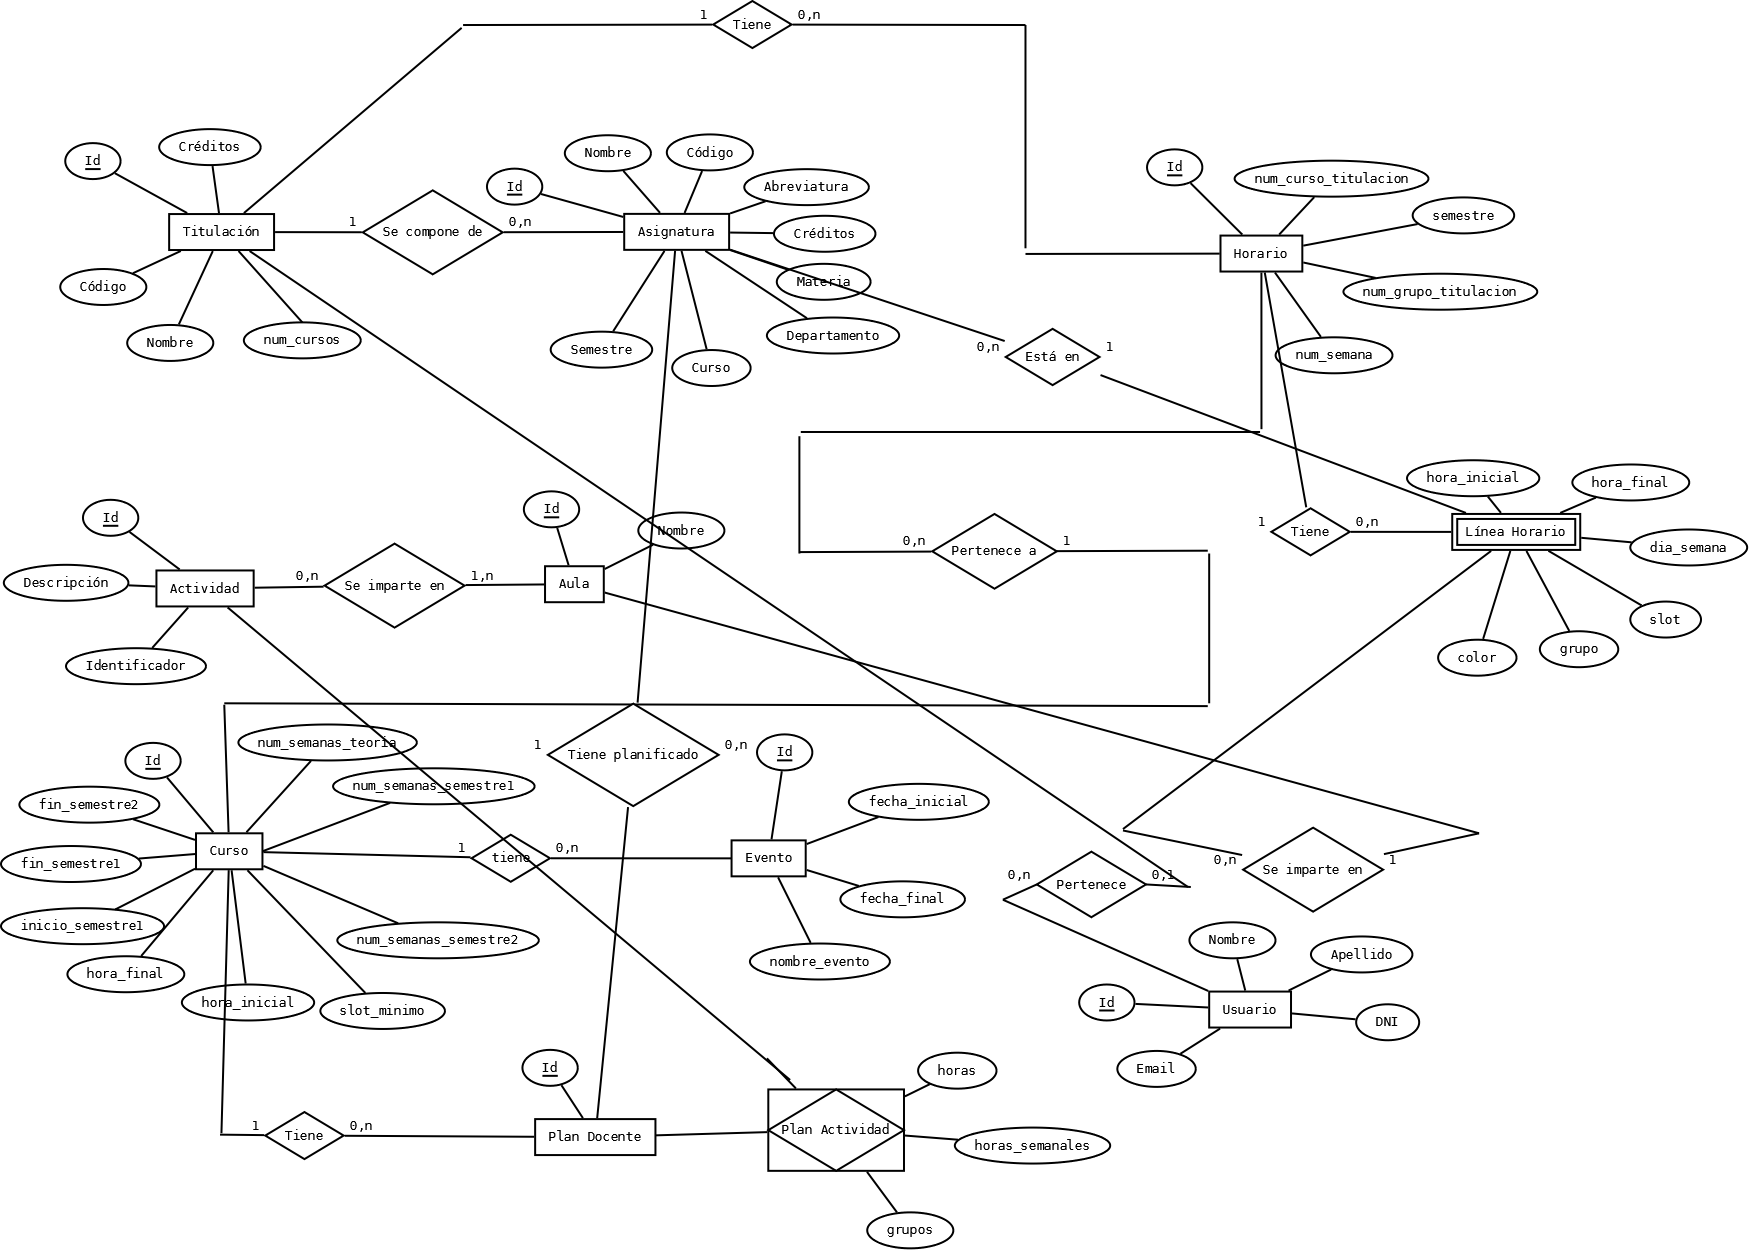
\includegraphics[scale=0.25,angle=90]{./ER.png}
  \end{center}
\caption{Diagrama Entidad-Relación}
\end{figure}
\subsection{Tablas y atributos}

% phpMyAdmin LaTeX Dump
% version 3.4.5
% http://www.phpmyadmin.net
%
% Servidor: localhost
% Tiempo de generación: 08-12-2011 a las 15:07:50
% Versión del servidor: 5.5.16
% Versión de PHP: 5.3.8
% 
% Base de datos: 'pfc_development'
% 

%
% Estructura: actividades
%
 \begin{longtable}{|l|c|c|c|} 
 \caption{Estructura de la tabla actividades} \label{tab:actividades-structure} \\
 \hline \multicolumn{1}{|c|}{\textbf{Columna}} & \multicolumn{1}{|c|}{\textbf{Tipo}} & \multicolumn{1}{|c|}{\textbf{Nulo}} & \multicolumn{1}{|c|}{\textbf{Predeterminado}} \\ \hline \hline
\endfirsthead
 \caption{Estructura de la tabla actividades (continúa)} \\ 
 \hline \multicolumn{1}{|c|}{\textbf{Columna}} & \multicolumn{1}{|c|}{\textbf{Tipo}} & \multicolumn{1}{|c|}{\textbf{Nulo}} & \multicolumn{1}{|c|}{\textbf{Predeterminado}} \\ \hline \hline \endhead \endfoot 
\textbf{\textit{id}} & bigint(20)  & No &  \\ \hline 
descripcion & varchar(100) & No &  \\ \hline 
identificador & varchar(1) & No &  \\ \hline 
 \end{longtable}

%
% Estructura: actividades
%
 \begin{longtable}{|l|c|c|c|} 
 \caption{Estructura de la tabla actividades} \label{tab:actividades-structure} \\
 \hline \multicolumn{1}{|c|}{\textbf{Columna}} & \multicolumn{1}{|c|}{\textbf{Tipo}} & \multicolumn{1}{|c|}{\textbf{Nulo}} & \multicolumn{1}{|c|}{\textbf{Predeterminado}} \\ \hline \hline
\endfirsthead
 \caption{Estructura de la tabla actividades (continúa)} \\ 
 \hline \multicolumn{1}{|c|}{\textbf{Columna}} & \multicolumn{1}{|c|}{\textbf{Tipo}} & \multicolumn{1}{|c|}{\textbf{Nulo}} & \multicolumn{1}{|c|}{\textbf{Predeterminado}} \\ \hline \hline \endhead \endfoot 
\textbf{\textit{id}} & bigint(20)  & No &  \\ \hline 
descripcion & varchar(100) & No &  \\ \hline 
identificador & varchar(1) & No &  \\ \hline 
 \end{longtable}

%
% Estructura: asignaturas
%
 \begin{longtable}{|l|c|c|c|l|} 
 \caption{Estructura de la tabla asignaturas} \label{tab:asignaturas-structure} \\
 \hline \multicolumn{1}{|c|}{\textbf{Columna}} & \multicolumn{1}{|c|}{\textbf{Tipo}} & \multicolumn{1}{|c|}{\textbf{Nulo}} & \multicolumn{1}{|c|}{\textbf{Predeterminado}} & \multicolumn{1}{|c|}{\textbf{Enlaces a}} \\ \hline \hline
\endfirsthead
 \caption{Estructura de la tabla asignaturas (continúa)} \\ 
 \hline \multicolumn{1}{|c|}{\textbf{Columna}} & \multicolumn{1}{|c|}{\textbf{Tipo}} & \multicolumn{1}{|c|}{\textbf{Nulo}} & \multicolumn{1}{|c|}{\textbf{Predeterminado}} & \multicolumn{1}{|c|}{\textbf{Enlaces a}} \\ \hline \hline \endhead \endfoot 
\textbf{\textit{id}} & int(11) & No &  &  \\ \hline 
\textbf{codigo} & varchar(3) & No &  &  \\ \hline 
nombre & varchar(200) & No &  &  \\ \hline 
abreviatura & varchar(5) & No &  &  \\ \hline 
creditos & int(11) & No &  &  \\ \hline 
materia & varchar(100) & No &  &  \\ \hline 
departamento & varchar(200) & No &  &  \\ \hline 
curso & int(10)  & No &  &  \\ \hline 
semestre & varchar(255) & No &  &  \\ \hline 
titulacion\_id & int(11) & No &  & titulaciones (id) \\ \hline 
 \end{longtable}

%
% Estructura: asignaturas
%
 \begin{longtable}{|l|c|c|c|l|} 
 \caption{Estructura de la tabla asignaturas} \label{tab:asignaturas-structure} \\
 \hline \multicolumn{1}{|c|}{\textbf{Columna}} & \multicolumn{1}{|c|}{\textbf{Tipo}} & \multicolumn{1}{|c|}{\textbf{Nulo}} & \multicolumn{1}{|c|}{\textbf{Predeterminado}} & \multicolumn{1}{|c|}{\textbf{Enlaces a}} \\ \hline \hline
\endfirsthead
 \caption{Estructura de la tabla asignaturas (continúa)} \\ 
 \hline \multicolumn{1}{|c|}{\textbf{Columna}} & \multicolumn{1}{|c|}{\textbf{Tipo}} & \multicolumn{1}{|c|}{\textbf{Nulo}} & \multicolumn{1}{|c|}{\textbf{Predeterminado}} & \multicolumn{1}{|c|}{\textbf{Enlaces a}} \\ \hline \hline \endhead \endfoot 
\textbf{\textit{id}} & int(11) & No &  &  \\ \hline 
\textbf{codigo} & varchar(3) & No &  &  \\ \hline 
nombre & varchar(200) & No &  &  \\ \hline 
abreviatura & varchar(5) & No &  &  \\ \hline 
creditos & int(11) & No &  &  \\ \hline 
materia & varchar(100) & No &  &  \\ \hline 
departamento & varchar(200) & No &  &  \\ \hline 
curso & int(10)  & No &  &  \\ \hline 
semestre & varchar(255) & No &  &  \\ \hline 
titulacion\_id & int(11) & No &  & titulaciones (id) \\ \hline 
 \end{longtable}

%
% Estructura: aulaactividades
%
 \begin{longtable}{|l|c|c|c|l|} 
 \caption{Estructura de la tabla aulaactividades} \label{tab:aulaactividades-structure} \\
 \hline \multicolumn{1}{|c|}{\textbf{Columna}} & \multicolumn{1}{|c|}{\textbf{Tipo}} & \multicolumn{1}{|c|}{\textbf{Nulo}} & \multicolumn{1}{|c|}{\textbf{Predeterminado}} & \multicolumn{1}{|c|}{\textbf{Enlaces a}} \\ \hline \hline
\endfirsthead
 \caption{Estructura de la tabla aulaactividades (continúa)} \\ 
 \hline \multicolumn{1}{|c|}{\textbf{Columna}} & \multicolumn{1}{|c|}{\textbf{Tipo}} & \multicolumn{1}{|c|}{\textbf{Nulo}} & \multicolumn{1}{|c|}{\textbf{Predeterminado}} & \multicolumn{1}{|c|}{\textbf{Enlaces a}} \\ \hline \hline \endhead \endfoot 
\textbf{\textit{id\_actividad}} & bigint(20)  & No &  & actividades (id) \\ \hline 
\textbf{\textit{id\_aula}} & bigint(20)  & No &  & aulas (id) \\ \hline 
 \end{longtable}

%
% Estructura: aulaactividades
%
 \begin{longtable}{|l|c|c|c|l|} 
 \caption{Estructura de la tabla aulaactividades} \label{tab:aulaactividades-structure} \\
 \hline \multicolumn{1}{|c|}{\textbf{Columna}} & \multicolumn{1}{|c|}{\textbf{Tipo}} & \multicolumn{1}{|c|}{\textbf{Nulo}} & \multicolumn{1}{|c|}{\textbf{Predeterminado}} & \multicolumn{1}{|c|}{\textbf{Enlaces a}} \\ \hline \hline
\endfirsthead
 \caption{Estructura de la tabla aulaactividades (continúa)} \\ 
 \hline \multicolumn{1}{|c|}{\textbf{Columna}} & \multicolumn{1}{|c|}{\textbf{Tipo}} & \multicolumn{1}{|c|}{\textbf{Nulo}} & \multicolumn{1}{|c|}{\textbf{Predeterminado}} & \multicolumn{1}{|c|}{\textbf{Enlaces a}} \\ \hline \hline \endhead \endfoot 
\textbf{\textit{id\_actividad}} & bigint(20)  & No &  & actividades (id) \\ \hline 
\textbf{\textit{id\_aula}} & bigint(20)  & No &  & aulas (id) \\ \hline 
 \end{longtable}

%
% Estructura: aulas
%
 \begin{longtable}{|l|c|c|c|} 
 \caption{Estructura de la tabla aulas} \label{tab:aulas-structure} \\
 \hline \multicolumn{1}{|c|}{\textbf{Columna}} & \multicolumn{1}{|c|}{\textbf{Tipo}} & \multicolumn{1}{|c|}{\textbf{Nulo}} & \multicolumn{1}{|c|}{\textbf{Predeterminado}} \\ \hline \hline
\endfirsthead
 \caption{Estructura de la tabla aulas (continúa)} \\ 
 \hline \multicolumn{1}{|c|}{\textbf{Columna}} & \multicolumn{1}{|c|}{\textbf{Tipo}} & \multicolumn{1}{|c|}{\textbf{Nulo}} & \multicolumn{1}{|c|}{\textbf{Predeterminado}} \\ \hline \hline \endhead \endfoot 
\textbf{\textit{id}} & bigint(20)  & No &  \\ \hline 
nombre & varchar(100) & No &  \\ \hline 
 \end{longtable}

%
% Estructura: aulas
%
 \begin{longtable}{|l|c|c|c|} 
 \caption{Estructura de la tabla aulas} \label{tab:aulas-structure} \\
 \hline \multicolumn{1}{|c|}{\textbf{Columna}} & \multicolumn{1}{|c|}{\textbf{Tipo}} & \multicolumn{1}{|c|}{\textbf{Nulo}} & \multicolumn{1}{|c|}{\textbf{Predeterminado}} \\ \hline \hline
\endfirsthead
 \caption{Estructura de la tabla aulas (continúa)} \\ 
 \hline \multicolumn{1}{|c|}{\textbf{Columna}} & \multicolumn{1}{|c|}{\textbf{Tipo}} & \multicolumn{1}{|c|}{\textbf{Nulo}} & \multicolumn{1}{|c|}{\textbf{Predeterminado}} \\ \hline \hline \endhead \endfoot 
\textbf{\textit{id}} & bigint(20)  & No &  \\ \hline 
nombre & varchar(100) & No &  \\ \hline 
 \end{longtable}

%
% Estructura: calendarios
%
 \begin{longtable}{|l|c|c|c|} 
 \caption{Estructura de la tabla calendarios} \label{tab:calendarios-structure} \\
 \hline \multicolumn{1}{|c|}{\textbf{Columna}} & \multicolumn{1}{|c|}{\textbf{Tipo}} & \multicolumn{1}{|c|}{\textbf{Nulo}} & \multicolumn{1}{|c|}{\textbf{Predeterminado}} \\ \hline \hline
\endfirsthead
 \caption{Estructura de la tabla calendarios (continúa)} \\ 
 \hline \multicolumn{1}{|c|}{\textbf{Columna}} & \multicolumn{1}{|c|}{\textbf{Tipo}} & \multicolumn{1}{|c|}{\textbf{Nulo}} & \multicolumn{1}{|c|}{\textbf{Predeterminado}} \\ \hline \hline \endhead \endfoot 
\textbf{\textit{id}} & int(11) & No &  \\ \hline 
\textbf{codigo} & varchar(4) & No &  \\ \hline 
 \end{longtable}

%
% Estructura: calendarios
%
 \begin{longtable}{|l|c|c|c|} 
 \caption{Estructura de la tabla calendarios} \label{tab:calendarios-structure} \\
 \hline \multicolumn{1}{|c|}{\textbf{Columna}} & \multicolumn{1}{|c|}{\textbf{Tipo}} & \multicolumn{1}{|c|}{\textbf{Nulo}} & \multicolumn{1}{|c|}{\textbf{Predeterminado}} \\ \hline \hline
\endfirsthead
 \caption{Estructura de la tabla calendarios (continúa)} \\ 
 \hline \multicolumn{1}{|c|}{\textbf{Columna}} & \multicolumn{1}{|c|}{\textbf{Tipo}} & \multicolumn{1}{|c|}{\textbf{Nulo}} & \multicolumn{1}{|c|}{\textbf{Predeterminado}} \\ \hline \hline \endhead \endfoot 
\textbf{\textit{id}} & int(11) & No &  \\ \hline 
\textbf{codigo} & varchar(4) & No &  \\ \hline 
 \end{longtable}

%
% Estructura: cargas_semanales
%
 \begin{longtable}{|l|c|c|c|l|} 
 \caption{Estructura de la tabla cargas\_semanales} \label{tab:cargas_semanales-structure} \\
 \hline \multicolumn{1}{|c|}{\textbf{Columna}} & \multicolumn{1}{|c|}{\textbf{Tipo}} & \multicolumn{1}{|c|}{\textbf{Nulo}} & \multicolumn{1}{|c|}{\textbf{Predeterminado}} & \multicolumn{1}{|c|}{\textbf{Enlaces a}} \\ \hline \hline
\endfirsthead
 \caption{Estructura de la tabla cargas\_semanales (continúa)} \\ 
 \hline \multicolumn{1}{|c|}{\textbf{Columna}} & \multicolumn{1}{|c|}{\textbf{Tipo}} & \multicolumn{1}{|c|}{\textbf{Nulo}} & \multicolumn{1}{|c|}{\textbf{Predeterminado}} & \multicolumn{1}{|c|}{\textbf{Enlaces a}} \\ \hline \hline \endhead \endfoot 
\textbf{\textit{id}} & int(11) & No &  &  \\ \hline 
num\_semana & int(10)  & No &  &  \\ \hline 
horas\_teoria & int(10)  & No &  &  \\ \hline 
horas\_problemas & int(10)  & No &  &  \\ \hline 
horas\_informatica & int(10)  & No &  &  \\ \hline 
horas\_lab & int(10)  & No &  &  \\ \hline 
horas\_campo & int(10)  & No &  &  \\ \hline 
entrega\_trabajo & tinyint(1) & No &  &  \\ \hline 
examen & tinyint(1) & No &  &  \\ \hline 
plandocente\_id & int(11) & No &  & planesdocentes (id) \\ \hline 
 \end{longtable}

%
% Estructura: cargas_semanales
%
 \begin{longtable}{|l|c|c|c|l|} 
 \caption{Estructura de la tabla cargas\_semanales} \label{tab:cargas_semanales-structure} \\
 \hline \multicolumn{1}{|c|}{\textbf{Columna}} & \multicolumn{1}{|c|}{\textbf{Tipo}} & \multicolumn{1}{|c|}{\textbf{Nulo}} & \multicolumn{1}{|c|}{\textbf{Predeterminado}} & \multicolumn{1}{|c|}{\textbf{Enlaces a}} \\ \hline \hline
\endfirsthead
 \caption{Estructura de la tabla cargas\_semanales (continúa)} \\ 
 \hline \multicolumn{1}{|c|}{\textbf{Columna}} & \multicolumn{1}{|c|}{\textbf{Tipo}} & \multicolumn{1}{|c|}{\textbf{Nulo}} & \multicolumn{1}{|c|}{\textbf{Predeterminado}} & \multicolumn{1}{|c|}{\textbf{Enlaces a}} \\ \hline \hline \endhead \endfoot 
\textbf{\textit{id}} & int(11) & No &  &  \\ \hline 
num\_semana & int(10)  & No &  &  \\ \hline 
horas\_teoria & int(10)  & No &  &  \\ \hline 
horas\_problemas & int(10)  & No &  &  \\ \hline 
horas\_informatica & int(10)  & No &  &  \\ \hline 
horas\_lab & int(10)  & No &  &  \\ \hline 
horas\_campo & int(10)  & No &  &  \\ \hline 
entrega\_trabajo & tinyint(1) & No &  &  \\ \hline 
examen & tinyint(1) & No &  &  \\ \hline 
plandocente\_id & int(11) & No &  & planesdocentes (id) \\ \hline 
 \end{longtable}

%
% Estructura: ci_sessions
%
 \begin{longtable}{|l|c|c|c|} 
 \caption{Estructura de la tabla ci\_sessions} \label{tab:ci_sessions-structure} \\
 \hline \multicolumn{1}{|c|}{\textbf{Columna}} & \multicolumn{1}{|c|}{\textbf{Tipo}} & \multicolumn{1}{|c|}{\textbf{Nulo}} & \multicolumn{1}{|c|}{\textbf{Predeterminado}} \\ \hline \hline
\endfirsthead
 \caption{Estructura de la tabla ci\_sessions (continúa)} \\ 
 \hline \multicolumn{1}{|c|}{\textbf{Columna}} & \multicolumn{1}{|c|}{\textbf{Tipo}} & \multicolumn{1}{|c|}{\textbf{Nulo}} & \multicolumn{1}{|c|}{\textbf{Predeterminado}} \\ \hline \hline \endhead \endfoot 
\textbf{\textit{session\_id}} & varchar(40) & No &  \\ \hline 
ip\_address & varchar(16) & No & 0 \\ \hline 
user\_agent & varchar(120) & No &  \\ \hline 
last\_activity & int(10)  & No & 0 \\ \hline 
user\_data & text & Sí & NULL \\ \hline 
 \end{longtable}

%
% Estructura: ci_sessions
%
 \begin{longtable}{|l|c|c|c|} 
 \caption{Estructura de la tabla ci\_sessions} \label{tab:ci_sessions-structure} \\
 \hline \multicolumn{1}{|c|}{\textbf{Columna}} & \multicolumn{1}{|c|}{\textbf{Tipo}} & \multicolumn{1}{|c|}{\textbf{Nulo}} & \multicolumn{1}{|c|}{\textbf{Predeterminado}} \\ \hline \hline
\endfirsthead
 \caption{Estructura de la tabla ci\_sessions (continúa)} \\ 
 \hline \multicolumn{1}{|c|}{\textbf{Columna}} & \multicolumn{1}{|c|}{\textbf{Tipo}} & \multicolumn{1}{|c|}{\textbf{Nulo}} & \multicolumn{1}{|c|}{\textbf{Predeterminado}} \\ \hline \hline \endhead \endfoot 
\textbf{\textit{session\_id}} & varchar(40) & No &  \\ \hline 
ip\_address & varchar(16) & No & 0 \\ \hline 
user\_agent & varchar(120) & No &  \\ \hline 
last\_activity & int(10)  & No & 0 \\ \hline 
user\_data & text & Sí & NULL \\ \hline 
 \end{longtable}

%
% Estructura: cursos
%
 \begin{longtable}{|l|c|c|c|} 
 \caption{Estructura de la tabla cursos} \label{tab:cursos-structure} \\
 \hline \multicolumn{1}{|c|}{\textbf{Columna}} & \multicolumn{1}{|c|}{\textbf{Tipo}} & \multicolumn{1}{|c|}{\textbf{Nulo}} & \multicolumn{1}{|c|}{\textbf{Predeterminado}} \\ \hline \hline
\endfirsthead
 \caption{Estructura de la tabla cursos (continúa)} \\ 
 \hline \multicolumn{1}{|c|}{\textbf{Columna}} & \multicolumn{1}{|c|}{\textbf{Tipo}} & \multicolumn{1}{|c|}{\textbf{Nulo}} & \multicolumn{1}{|c|}{\textbf{Predeterminado}} \\ \hline \hline \endhead \endfoot 
\textbf{\textit{id}} & int(11) & No &  \\ \hline 
num\_semanas\_teoria & int(11) & No &  \\ \hline 
num\_semanas\_semestre1 & int(11) & No & 0 \\ \hline 
num\_semanas\_semestre2 & int(11) & No & 0 \\ \hline 
horas\_por\_credito & int(11) & No &  \\ \hline 
slot\_minimo & bigint(20) & No & 30 \\ \hline 
hora\_inicial & time & No & 09:00:00 \\ \hline 
hora\_final & time & No & 22:00:00 \\ \hline 
inicio\_semestre1 & date & No &  \\ \hline 
fin\_semestre1 & date & No &  \\ \hline 
inicio\_semestre2 & date & No &  \\ \hline 
fin\_semestre2 & date & No &  \\ \hline 
inicio\_examenes\_enero & date & No &  \\ \hline 
fin\_examenes\_enero & date & No &  \\ \hline 
inicio\_examenes\_junio & date & No &  \\ \hline 
fin\_examenes\_junio & date & No &  \\ \hline 
inicio\_examenes\_sept & date & No &  \\ \hline 
fin\_examenes\_sept & date & No &  \\ \hline 
 \end{longtable}

%
% Estructura: cursos
%
 \begin{longtable}{|l|c|c|c|} 
 \caption{Estructura de la tabla cursos} \label{tab:cursos-structure} \\
 \hline \multicolumn{1}{|c|}{\textbf{Columna}} & \multicolumn{1}{|c|}{\textbf{Tipo}} & \multicolumn{1}{|c|}{\textbf{Nulo}} & \multicolumn{1}{|c|}{\textbf{Predeterminado}} \\ \hline \hline
\endfirsthead
 \caption{Estructura de la tabla cursos (continúa)} \\ 
 \hline \multicolumn{1}{|c|}{\textbf{Columna}} & \multicolumn{1}{|c|}{\textbf{Tipo}} & \multicolumn{1}{|c|}{\textbf{Nulo}} & \multicolumn{1}{|c|}{\textbf{Predeterminado}} \\ \hline \hline \endhead \endfoot 
\textbf{\textit{id}} & int(11) & No &  \\ \hline 
num\_semanas\_teoria & int(11) & No &  \\ \hline 
num\_semanas\_semestre1 & int(11) & No & 0 \\ \hline 
num\_semanas\_semestre2 & int(11) & No & 0 \\ \hline 
horas\_por\_credito & int(11) & No &  \\ \hline 
slot\_minimo & bigint(20) & No & 30 \\ \hline 
hora\_inicial & time & No & 09:00:00 \\ \hline 
hora\_final & time & No & 22:00:00 \\ \hline 
inicio\_semestre1 & date & No &  \\ \hline 
fin\_semestre1 & date & No &  \\ \hline 
inicio\_semestre2 & date & No &  \\ \hline 
fin\_semestre2 & date & No &  \\ \hline 
inicio\_examenes\_enero & date & No &  \\ \hline 
fin\_examenes\_enero & date & No &  \\ \hline 
inicio\_examenes\_junio & date & No &  \\ \hline 
fin\_examenes\_junio & date & No &  \\ \hline 
inicio\_examenes\_sept & date & No &  \\ \hline 
fin\_examenes\_sept & date & No &  \\ \hline 
 \end{longtable}

%
% Estructura: cursos_compartidos
%
 \begin{longtable}{|l|c|c|c|l|} 
 \caption{Estructura de la tabla cursos\_compartidos} \label{tab:cursos_compartidos-structure} \\
 \hline \multicolumn{1}{|c|}{\textbf{Columna}} & \multicolumn{1}{|c|}{\textbf{Tipo}} & \multicolumn{1}{|c|}{\textbf{Nulo}} & \multicolumn{1}{|c|}{\textbf{Predeterminado}} & \multicolumn{1}{|c|}{\textbf{Enlaces a}} \\ \hline \hline
\endfirsthead
 \caption{Estructura de la tabla cursos\_compartidos (continúa)} \\ 
 \hline \multicolumn{1}{|c|}{\textbf{Columna}} & \multicolumn{1}{|c|}{\textbf{Tipo}} & \multicolumn{1}{|c|}{\textbf{Nulo}} & \multicolumn{1}{|c|}{\textbf{Predeterminado}} & \multicolumn{1}{|c|}{\textbf{Enlaces a}} \\ \hline \hline \endhead \endfoot 
\textbf{\textit{id\_plandocente}} & int(11) & No &  & planesdocentes (id) \\ \hline 
\textbf{\textit{num\_curso\_compartido}} & int(11) & No &  &  \\ \hline 
 \end{longtable}

%
% Estructura: cursos_compartidos
%
 \begin{longtable}{|l|c|c|c|l|} 
 \caption{Estructura de la tabla cursos\_compartidos} \label{tab:cursos_compartidos-structure} \\
 \hline \multicolumn{1}{|c|}{\textbf{Columna}} & \multicolumn{1}{|c|}{\textbf{Tipo}} & \multicolumn{1}{|c|}{\textbf{Nulo}} & \multicolumn{1}{|c|}{\textbf{Predeterminado}} & \multicolumn{1}{|c|}{\textbf{Enlaces a}} \\ \hline \hline
\endfirsthead
 \caption{Estructura de la tabla cursos\_compartidos (continúa)} \\ 
 \hline \multicolumn{1}{|c|}{\textbf{Columna}} & \multicolumn{1}{|c|}{\textbf{Tipo}} & \multicolumn{1}{|c|}{\textbf{Nulo}} & \multicolumn{1}{|c|}{\textbf{Predeterminado}} & \multicolumn{1}{|c|}{\textbf{Enlaces a}} \\ \hline \hline \endhead \endfoot 
\textbf{\textit{id\_plandocente}} & int(11) & No &  & planesdocentes (id) \\ \hline 
\textbf{\textit{num\_curso\_compartido}} & int(11) & No &  &  \\ \hline 
 \end{longtable}

%
% Estructura: eventos
%
 \begin{longtable}{|l|c|c|c|l|} 
 \caption{Estructura de la tabla eventos} \label{tab:eventos-structure} \\
 \hline \multicolumn{1}{|c|}{\textbf{Columna}} & \multicolumn{1}{|c|}{\textbf{Tipo}} & \multicolumn{1}{|c|}{\textbf{Nulo}} & \multicolumn{1}{|c|}{\textbf{Predeterminado}} & \multicolumn{1}{|c|}{\textbf{Enlaces a}} \\ \hline \hline
\endfirsthead
 \caption{Estructura de la tabla eventos (continúa)} \\ 
 \hline \multicolumn{1}{|c|}{\textbf{Columna}} & \multicolumn{1}{|c|}{\textbf{Tipo}} & \multicolumn{1}{|c|}{\textbf{Nulo}} & \multicolumn{1}{|c|}{\textbf{Predeterminado}} & \multicolumn{1}{|c|}{\textbf{Enlaces a}} \\ \hline \hline \endhead \endfoot 
\textbf{\textit{id}} & int(11) & No &  &  \\ \hline 
nombre\_evento & varchar(255) & No &  &  \\ \hline 
tipo\_evento & varchar(255) & No &  &  \\ \hline 
fecha\_individual & tinyint(1) & No &  &  \\ \hline 
fecha\_inicial & date & No &  &  \\ \hline 
fecha\_final & date & No &  &  \\ \hline 
curso\_id & int(11) & No &  & cursos (id) \\ \hline 
 \end{longtable}

%
% Estructura: eventos
%
 \begin{longtable}{|l|c|c|c|l|} 
 \caption{Estructura de la tabla eventos} \label{tab:eventos-structure} \\
 \hline \multicolumn{1}{|c|}{\textbf{Columna}} & \multicolumn{1}{|c|}{\textbf{Tipo}} & \multicolumn{1}{|c|}{\textbf{Nulo}} & \multicolumn{1}{|c|}{\textbf{Predeterminado}} & \multicolumn{1}{|c|}{\textbf{Enlaces a}} \\ \hline \hline
\endfirsthead
 \caption{Estructura de la tabla eventos (continúa)} \\ 
 \hline \multicolumn{1}{|c|}{\textbf{Columna}} & \multicolumn{1}{|c|}{\textbf{Tipo}} & \multicolumn{1}{|c|}{\textbf{Nulo}} & \multicolumn{1}{|c|}{\textbf{Predeterminado}} & \multicolumn{1}{|c|}{\textbf{Enlaces a}} \\ \hline \hline \endhead \endfoot 
\textbf{\textit{id}} & int(11) & No &  &  \\ \hline 
nombre\_evento & varchar(255) & No &  &  \\ \hline 
tipo\_evento & varchar(255) & No &  &  \\ \hline 
fecha\_individual & tinyint(1) & No &  &  \\ \hline 
fecha\_inicial & date & No &  &  \\ \hline 
fecha\_final & date & No &  &  \\ \hline 
curso\_id & int(11) & No &  & cursos (id) \\ \hline 
 \end{longtable}

%
% Estructura: horarios
%
 \begin{longtable}{|l|c|c|c|l|} 
 \caption{Estructura de la tabla horarios} \label{tab:horarios-structure} \\
 \hline \multicolumn{1}{|c|}{\textbf{Columna}} & \multicolumn{1}{|c|}{\textbf{Tipo}} & \multicolumn{1}{|c|}{\textbf{Nulo}} & \multicolumn{1}{|c|}{\textbf{Predeterminado}} & \multicolumn{1}{|c|}{\textbf{Enlaces a}} \\ \hline \hline
\endfirsthead
 \caption{Estructura de la tabla horarios (continúa)} \\ 
 \hline \multicolumn{1}{|c|}{\textbf{Columna}} & \multicolumn{1}{|c|}{\textbf{Tipo}} & \multicolumn{1}{|c|}{\textbf{Nulo}} & \multicolumn{1}{|c|}{\textbf{Predeterminado}} & \multicolumn{1}{|c|}{\textbf{Enlaces a}} \\ \hline \hline \endhead \endfoot 
\textbf{\textit{id}} & int(11) & No &  &  \\ \hline 
id\_curso & int(11) & No &  & cursos (id) \\ \hline 
id\_titulacion & int(11) & No &  & titulaciones (id) \\ \hline 
num\_curso\_titulacion & int(11) & No &  &  \\ \hline 
semestre & varchar(255) & No &  &  \\ \hline 
num\_grupo\_titulacion & int(11) & No &  &  \\ \hline 
num\_semana & int(10)  & No &  &  \\ \hline 
 \end{longtable}

%
% Estructura: horarios
%
 \begin{longtable}{|l|c|c|c|l|} 
 \caption{Estructura de la tabla horarios} \label{tab:horarios-structure} \\
 \hline \multicolumn{1}{|c|}{\textbf{Columna}} & \multicolumn{1}{|c|}{\textbf{Tipo}} & \multicolumn{1}{|c|}{\textbf{Nulo}} & \multicolumn{1}{|c|}{\textbf{Predeterminado}} & \multicolumn{1}{|c|}{\textbf{Enlaces a}} \\ \hline \hline
\endfirsthead
 \caption{Estructura de la tabla horarios (continúa)} \\ 
 \hline \multicolumn{1}{|c|}{\textbf{Columna}} & \multicolumn{1}{|c|}{\textbf{Tipo}} & \multicolumn{1}{|c|}{\textbf{Nulo}} & \multicolumn{1}{|c|}{\textbf{Predeterminado}} & \multicolumn{1}{|c|}{\textbf{Enlaces a}} \\ \hline \hline \endhead \endfoot 
\textbf{\textit{id}} & int(11) & No &  &  \\ \hline 
id\_curso & int(11) & No &  & cursos (id) \\ \hline 
id\_titulacion & int(11) & No &  & titulaciones (id) \\ \hline 
num\_curso\_titulacion & int(11) & No &  &  \\ \hline 
semestre & varchar(255) & No &  &  \\ \hline 
num\_grupo\_titulacion & int(11) & No &  &  \\ \hline 
num\_semana & int(10)  & No &  &  \\ \hline 
 \end{longtable}

%
% Estructura: horario_reference
%
 \begin{longtable}{|l|c|c|c|} 
 \caption{Estructura de la tabla horario\_reference} \label{tab:horario_reference-structure} \\
 \hline \multicolumn{1}{|c|}{\textbf{Columna}} & \multicolumn{1}{|c|}{\textbf{Tipo}} & \multicolumn{1}{|c|}{\textbf{Nulo}} & \multicolumn{1}{|c|}{\textbf{Predeterminado}} \\ \hline \hline
\endfirsthead
 \caption{Estructura de la tabla horario\_reference (continúa)} \\ 
 \hline \multicolumn{1}{|c|}{\textbf{Columna}} & \multicolumn{1}{|c|}{\textbf{Tipo}} & \multicolumn{1}{|c|}{\textbf{Nulo}} & \multicolumn{1}{|c|}{\textbf{Predeterminado}} \\ \hline \hline \endhead \endfoot 
\textbf{\textit{id\_tipo}} & bigint(20)  & No &  \\ \hline 
\textbf{\textit{id\_teoria}} & bigint(20)  & No &  \\ \hline 
 \end{longtable}

%
% Estructura: horario_reference
%
 \begin{longtable}{|l|c|c|c|} 
 \caption{Estructura de la tabla horario\_reference} \label{tab:horario_reference-structure} \\
 \hline \multicolumn{1}{|c|}{\textbf{Columna}} & \multicolumn{1}{|c|}{\textbf{Tipo}} & \multicolumn{1}{|c|}{\textbf{Nulo}} & \multicolumn{1}{|c|}{\textbf{Predeterminado}} \\ \hline \hline
\endfirsthead
 \caption{Estructura de la tabla horario\_reference (continúa)} \\ 
 \hline \multicolumn{1}{|c|}{\textbf{Columna}} & \multicolumn{1}{|c|}{\textbf{Tipo}} & \multicolumn{1}{|c|}{\textbf{Nulo}} & \multicolumn{1}{|c|}{\textbf{Predeterminado}} \\ \hline \hline \endhead \endfoot 
\textbf{\textit{id\_tipo}} & bigint(20)  & No &  \\ \hline 
\textbf{\textit{id\_teoria}} & bigint(20)  & No &  \\ \hline 
 \end{longtable}

%
% Estructura: lineashorarios
%
 \begin{longtable}{|l|c|c|c|l|} 
 \caption{Estructura de la tabla lineashorarios} \label{tab:lineashorarios-structure} \\
 \hline \multicolumn{1}{|c|}{\textbf{Columna}} & \multicolumn{1}{|c|}{\textbf{Tipo}} & \multicolumn{1}{|c|}{\textbf{Nulo}} & \multicolumn{1}{|c|}{\textbf{Predeterminado}} & \multicolumn{1}{|c|}{\textbf{Enlaces a}} \\ \hline \hline
\endfirsthead
 \caption{Estructura de la tabla lineashorarios (continúa)} \\ 
 \hline \multicolumn{1}{|c|}{\textbf{Columna}} & \multicolumn{1}{|c|}{\textbf{Tipo}} & \multicolumn{1}{|c|}{\textbf{Nulo}} & \multicolumn{1}{|c|}{\textbf{Predeterminado}} & \multicolumn{1}{|c|}{\textbf{Enlaces a}} \\ \hline \hline \endhead \endfoot 
\textbf{\textit{id}} & int(11) & No &  &  \\ \hline 
id\_horario & int(11) & No &  & horarios (id) \\ \hline 
id\_asignatura & int(11) & No &  & asignaturas (id) \\ \hline 
hora\_inicial & time & Sí & NULL &  \\ \hline 
hora\_final & time & Sí & NULL &  \\ \hline 
dia\_semana & tinyint(3)  & Sí & NULL &  \\ \hline 
id\_actividad & bigint(20)  & Sí & NULL & actividades (id) \\ \hline 
num\_grupo\_actividad & bigint(20)  & No &  &  \\ \hline 
slot\_minimo & float(18,2) & No &  &  \\ \hline 
color & varchar(7) & Sí & NULL &  \\ \hline 
id\_aula & bigint(20)  & Sí & NULL & aulas (id) \\ \hline 
 \end{longtable}

%
% Estructura: lineashorarios
%
 \begin{longtable}{|l|c|c|c|l|} 
 \caption{Estructura de la tabla lineashorarios} \label{tab:lineashorarios-structure} \\
 \hline \multicolumn{1}{|c|}{\textbf{Columna}} & \multicolumn{1}{|c|}{\textbf{Tipo}} & \multicolumn{1}{|c|}{\textbf{Nulo}} & \multicolumn{1}{|c|}{\textbf{Predeterminado}} & \multicolumn{1}{|c|}{\textbf{Enlaces a}} \\ \hline \hline
\endfirsthead
 \caption{Estructura de la tabla lineashorarios (continúa)} \\ 
 \hline \multicolumn{1}{|c|}{\textbf{Columna}} & \multicolumn{1}{|c|}{\textbf{Tipo}} & \multicolumn{1}{|c|}{\textbf{Nulo}} & \multicolumn{1}{|c|}{\textbf{Predeterminado}} & \multicolumn{1}{|c|}{\textbf{Enlaces a}} \\ \hline \hline \endhead \endfoot 
\textbf{\textit{id}} & int(11) & No &  &  \\ \hline 
id\_horario & int(11) & No &  & horarios (id) \\ \hline 
id\_asignatura & int(11) & No &  & asignaturas (id) \\ \hline 
hora\_inicial & time & Sí & NULL &  \\ \hline 
hora\_final & time & Sí & NULL &  \\ \hline 
dia\_semana & tinyint(3)  & Sí & NULL &  \\ \hline 
id\_actividad & bigint(20)  & Sí & NULL & actividades (id) \\ \hline 
num\_grupo\_actividad & bigint(20)  & No &  &  \\ \hline 
slot\_minimo & float(18,2) & No &  &  \\ \hline 
color & varchar(7) & Sí & NULL &  \\ \hline 
id\_aula & bigint(20)  & Sí & NULL & aulas (id) \\ \hline 
 \end{longtable}

%
% Estructura: planactividades
%
 \begin{longtable}{|l|c|c|c|l|} 
 \caption{Estructura de la tabla planactividades} \label{tab:planactividades-structure} \\
 \hline \multicolumn{1}{|c|}{\textbf{Columna}} & \multicolumn{1}{|c|}{\textbf{Tipo}} & \multicolumn{1}{|c|}{\textbf{Nulo}} & \multicolumn{1}{|c|}{\textbf{Predeterminado}} & \multicolumn{1}{|c|}{\textbf{Enlaces a}} \\ \hline \hline
\endfirsthead
 \caption{Estructura de la tabla planactividades (continúa)} \\ 
 \hline \multicolumn{1}{|c|}{\textbf{Columna}} & \multicolumn{1}{|c|}{\textbf{Tipo}} & \multicolumn{1}{|c|}{\textbf{Nulo}} & \multicolumn{1}{|c|}{\textbf{Predeterminado}} & \multicolumn{1}{|c|}{\textbf{Enlaces a}} \\ \hline \hline \endhead \endfoot 
\textbf{\textit{id}} & int(11) & No &  &  \\ \hline 
id\_plandocente & int(11) & No &  & planesdocentes (id) \\ \hline 
id\_actividad & bigint(20)  & No &  & actividades (id) \\ \hline 
horas & int(10)  & No & 0 &  \\ \hline 
grupos & int(10)  & No & 0 &  \\ \hline 
horas\_semanales & int(10)  & No & 0 &  \\ \hline 
alternas & tinyint(1) & Sí & NULL &  \\ \hline 
 \end{longtable}

%
% Estructura: planactividades
%
 \begin{longtable}{|l|c|c|c|l|} 
 \caption{Estructura de la tabla planactividades} \label{tab:planactividades-structure} \\
 \hline \multicolumn{1}{|c|}{\textbf{Columna}} & \multicolumn{1}{|c|}{\textbf{Tipo}} & \multicolumn{1}{|c|}{\textbf{Nulo}} & \multicolumn{1}{|c|}{\textbf{Predeterminado}} & \multicolumn{1}{|c|}{\textbf{Enlaces a}} \\ \hline \hline
\endfirsthead
 \caption{Estructura de la tabla planactividades (continúa)} \\ 
 \hline \multicolumn{1}{|c|}{\textbf{Columna}} & \multicolumn{1}{|c|}{\textbf{Tipo}} & \multicolumn{1}{|c|}{\textbf{Nulo}} & \multicolumn{1}{|c|}{\textbf{Predeterminado}} & \multicolumn{1}{|c|}{\textbf{Enlaces a}} \\ \hline \hline \endhead \endfoot 
\textbf{\textit{id}} & int(11) & No &  &  \\ \hline 
id\_plandocente & int(11) & No &  & planesdocentes (id) \\ \hline 
id\_actividad & bigint(20)  & No &  & actividades (id) \\ \hline 
horas & int(10)  & No & 0 &  \\ \hline 
grupos & int(10)  & No & 0 &  \\ \hline 
horas\_semanales & int(10)  & No & 0 &  \\ \hline 
alternas & tinyint(1) & Sí & NULL &  \\ \hline 
 \end{longtable}

%
% Estructura: planesdocentes
%
 \begin{longtable}{|l|c|c|c|l|} 
 \caption{Estructura de la tabla planesdocentes} \label{tab:planesdocentes-structure} \\
 \hline \multicolumn{1}{|c|}{\textbf{Columna}} & \multicolumn{1}{|c|}{\textbf{Tipo}} & \multicolumn{1}{|c|}{\textbf{Nulo}} & \multicolumn{1}{|c|}{\textbf{Predeterminado}} & \multicolumn{1}{|c|}{\textbf{Enlaces a}} \\ \hline \hline
\endfirsthead
 \caption{Estructura de la tabla planesdocentes (continúa)} \\ 
 \hline \multicolumn{1}{|c|}{\textbf{Columna}} & \multicolumn{1}{|c|}{\textbf{Tipo}} & \multicolumn{1}{|c|}{\textbf{Nulo}} & \multicolumn{1}{|c|}{\textbf{Predeterminado}} & \multicolumn{1}{|c|}{\textbf{Enlaces a}} \\ \hline \hline \endhead \endfoot 
\textbf{\textit{id}} & int(11) & No &  &  \\ \hline 
id\_asignatura & int(11) & No &  & asignaturas (id) \\ \hline 
id\_curso & int(11) & No &  & cursos (id) \\ \hline 
 \end{longtable}

%
% Estructura: planesdocentes
%
 \begin{longtable}{|l|c|c|c|l|} 
 \caption{Estructura de la tabla planesdocentes} \label{tab:planesdocentes-structure} \\
 \hline \multicolumn{1}{|c|}{\textbf{Columna}} & \multicolumn{1}{|c|}{\textbf{Tipo}} & \multicolumn{1}{|c|}{\textbf{Nulo}} & \multicolumn{1}{|c|}{\textbf{Predeterminado}} & \multicolumn{1}{|c|}{\textbf{Enlaces a}} \\ \hline \hline
\endfirsthead
 \caption{Estructura de la tabla planesdocentes (continúa)} \\ 
 \hline \multicolumn{1}{|c|}{\textbf{Columna}} & \multicolumn{1}{|c|}{\textbf{Tipo}} & \multicolumn{1}{|c|}{\textbf{Nulo}} & \multicolumn{1}{|c|}{\textbf{Predeterminado}} & \multicolumn{1}{|c|}{\textbf{Enlaces a}} \\ \hline \hline \endhead \endfoot 
\textbf{\textit{id}} & int(11) & No &  &  \\ \hline 
id\_asignatura & int(11) & No &  & asignaturas (id) \\ \hline 
id\_curso & int(11) & No &  & cursos (id) \\ \hline 
 \end{longtable}

%
% Estructura: titulaciones
%
 \begin{longtable}{|l|c|c|c|} 
 \caption{Estructura de la tabla titulaciones} \label{tab:titulaciones-structure} \\
 \hline \multicolumn{1}{|c|}{\textbf{Columna}} & \multicolumn{1}{|c|}{\textbf{Tipo}} & \multicolumn{1}{|c|}{\textbf{Nulo}} & \multicolumn{1}{|c|}{\textbf{Predeterminado}} \\ \hline \hline
\endfirsthead
 \caption{Estructura de la tabla titulaciones (continúa)} \\ 
 \hline \multicolumn{1}{|c|}{\textbf{Columna}} & \multicolumn{1}{|c|}{\textbf{Tipo}} & \multicolumn{1}{|c|}{\textbf{Nulo}} & \multicolumn{1}{|c|}{\textbf{Predeterminado}} \\ \hline \hline \endhead \endfoot 
\textbf{\textit{id}} & int(11) & No &  \\ \hline 
\textbf{codigo} & varchar(4) & No &  \\ \hline 
\textbf{nombre} & varchar(200) & No &  \\ \hline 
creditos & int(10)  & No &  \\ \hline 
num\_cursos & int(10)  & No &  \\ \hline 
 \end{longtable}

%
% Estructura: titulaciones
%
 \begin{longtable}{|l|c|c|c|} 
 \caption{Estructura de la tabla titulaciones} \label{tab:titulaciones-structure} \\
 \hline \multicolumn{1}{|c|}{\textbf{Columna}} & \multicolumn{1}{|c|}{\textbf{Tipo}} & \multicolumn{1}{|c|}{\textbf{Nulo}} & \multicolumn{1}{|c|}{\textbf{Predeterminado}} \\ \hline \hline
\endfirsthead
 \caption{Estructura de la tabla titulaciones (continúa)} \\ 
 \hline \multicolumn{1}{|c|}{\textbf{Columna}} & \multicolumn{1}{|c|}{\textbf{Tipo}} & \multicolumn{1}{|c|}{\textbf{Nulo}} & \multicolumn{1}{|c|}{\textbf{Predeterminado}} \\ \hline \hline \endhead \endfoot 
\textbf{\textit{id}} & int(11) & No &  \\ \hline 
\textbf{codigo} & varchar(4) & No &  \\ \hline 
\textbf{nombre} & varchar(200) & No &  \\ \hline 
creditos & int(10)  & No &  \\ \hline 
num\_cursos & int(10)  & No &  \\ \hline 
 \end{longtable}

%
% Estructura: users
%
 \begin{longtable}{|l|c|c|c|l|} 
 \caption{Estructura de la tabla users} \label{tab:users-structure} \\
 \hline \multicolumn{1}{|c|}{\textbf{Columna}} & \multicolumn{1}{|c|}{\textbf{Tipo}} & \multicolumn{1}{|c|}{\textbf{Nulo}} & \multicolumn{1}{|c|}{\textbf{Predeterminado}} & \multicolumn{1}{|c|}{\textbf{Enlaces a}} \\ \hline \hline
\endfirsthead
 \caption{Estructura de la tabla users (continúa)} \\ 
 \hline \multicolumn{1}{|c|}{\textbf{Columna}} & \multicolumn{1}{|c|}{\textbf{Tipo}} & \multicolumn{1}{|c|}{\textbf{Nulo}} & \multicolumn{1}{|c|}{\textbf{Predeterminado}} & \multicolumn{1}{|c|}{\textbf{Enlaces a}} \\ \hline \hline \endhead \endfoot 
\textbf{\textit{id}} & int(11) & No &  &  \\ \hline 
password & varchar(255) & No &  &  \\ \hline 
nombre & varchar(50) & No &  &  \\ \hline 
apellidos & varchar(50) & No &  &  \\ \hline 
\textbf{dni} & varchar(9) & No &  &  \\ \hline 
\textbf{email} & varchar(30) & No &  &  \\ \hline 
id\_titulacion & int(11) & No &  & titulaciones (id) \\ \hline 
level & int(10)  & No & 0 &  \\ \hline 
 \end{longtable}

%
% Estructura: users
%
 \begin{longtable}{|l|c|c|c|l|} 
 \caption{Estructura de la tabla users} \label{tab:users-structure} \\
 \hline \multicolumn{1}{|c|}{\textbf{Columna}} & \multicolumn{1}{|c|}{\textbf{Tipo}} & \multicolumn{1}{|c|}{\textbf{Nulo}} & \multicolumn{1}{|c|}{\textbf{Predeterminado}} & \multicolumn{1}{|c|}{\textbf{Enlaces a}} \\ \hline \hline
\endfirsthead
 \caption{Estructura de la tabla users (continúa)} \\ 
 \hline \multicolumn{1}{|c|}{\textbf{Columna}} & \multicolumn{1}{|c|}{\textbf{Tipo}} & \multicolumn{1}{|c|}{\textbf{Nulo}} & \multicolumn{1}{|c|}{\textbf{Predeterminado}} & \multicolumn{1}{|c|}{\textbf{Enlaces a}} \\ \hline \hline \endhead \endfoot 
\textbf{\textit{id}} & int(11) & No &  &  \\ \hline 
password & varchar(255) & No &  &  \\ \hline 
nombre & varchar(50) & No &  &  \\ \hline 
apellidos & varchar(50) & No &  &  \\ \hline 
\textbf{dni} & varchar(9) & No &  &  \\ \hline 
\textbf{email} & varchar(30) & No &  &  \\ \hline 
id\_titulacion & int(11) & No &  & titulaciones (id) \\ \hline 
level & int(10)  & No & 0 &  \\ \hline 
 \end{longtable}
